\chapter{Related Work}

In this section we explore some tools and techniques related to the processes described in our work. We have decided to divide this section into: Product, Process and Automation. Product describes an alternative solution to the utilized automation tool (Team Foundation Server/Azure DevOps). Jenkins is one of the most popular applications for the implementation of continuous integration/delivery/deployment techniques and it constitutes an interesting object of study given its open source nature as opposed to the closed source TFS. The completely customizable extensibility of Jenkis with the use of plugins is another characteristic that further motivated this initial comparison. Process elaborates on the concept of Behavioral Testing (and Behavior-Driven Development), and on a possible tool (Cucumber) to employ said techniques. We have decided to introduce the notion of BDD in order to describe a viable approach for the company to develop future applications with a major focus not only on the concept of testing but also on the communication between developers, consultants and key users. This technique, while not directly utilized during the course of this project, may represents a key step for the improvement of the quality and quantity of testing techniques applied during a project development. Because of this reason we believed it to be worthy of description. Finally, Automation gives some background information regarding the notion of Continuous Integration. We decided to provide a brief introduction in this regard because of the fact that CI constitutes the basis for the employment of regression testing techniques which represent one of the final objectives of this work.

%********************************** %First Section  **************************************
\section{Product} 

Jenkins \cite{JenkinsGuide} is a java-based, open-source automation software released under the MIT License. The extreme flexibility of the software makes it adaptable to a very wide range of requirements such as version control, code quality monitoring, testing, build tools, etc.
The tool can be extended with thousands of available open source plugins that can also be used to integrate various DevOps techniques. Jenkins can be executed as a Java servlet in a container (like Apache Tomcat) or using its own container application, called Jetty \cite[p.~51]{JenkinsGuide}. Jenkins comes with an array of Built-In Tool Providers (Apache Ant, GIT, JDK, Maven) that can be expanded by installing additional plugins either from the web UI or by using the CLI command \textit{install-plugin}. Jenkins is often used as a Continuous Integration / Continuous Delivery tool. Continuous Deployment is also achievable but often times more conservative approaches (such as a manual one-click deployment) are preferred by companies in order to have a more direct control over the process \cite[p.~325]{JenkinsGuide}. A suite of plugins that enables the use of Continuous Delivery techniques is called a Jenkins Pipeline [Figure \ref{fig:jenkinsPipeline}]. Said pipelines are fundamentally a series of repeatable interlinked steps that may allow changes in the code to be automatically deployed. This chain of scripts provides various benefits \cite[p.~165]{JenkinsCD} such as:

\begin{itemize}
  \item Grouping of operations. Operations are organized together into clearly defined stages. If one of such stages fails, the process is interrupted.
  \item Visibility. All aspects of the process are clearly visible.
  \item Feedback. Problems in the process are immediately reported.
\end{itemize}

Jenkins pipelines are composed by two kind of elements \cite[p.~166]{JenkinsCD}: stages and steps. A step is a minimal operation that tells the software to perform an action (like executing a script). A stage is a group of logically related steps (like building). Pipelines can be written directly in Jenkins or can be created in text files called JenkinsFile \cite[p.~186]{JenkinsCD} where the single steps are defined.
Benefits of using said files include prevention of data loss (pipelines definitions are stored in the repository), code quality improvement (code reviews) and security (access restrictions are the same as the ones used for the source code). The syntax used in these files may be declarative or scripted.

\begin{figure}[ht]
	\centering
	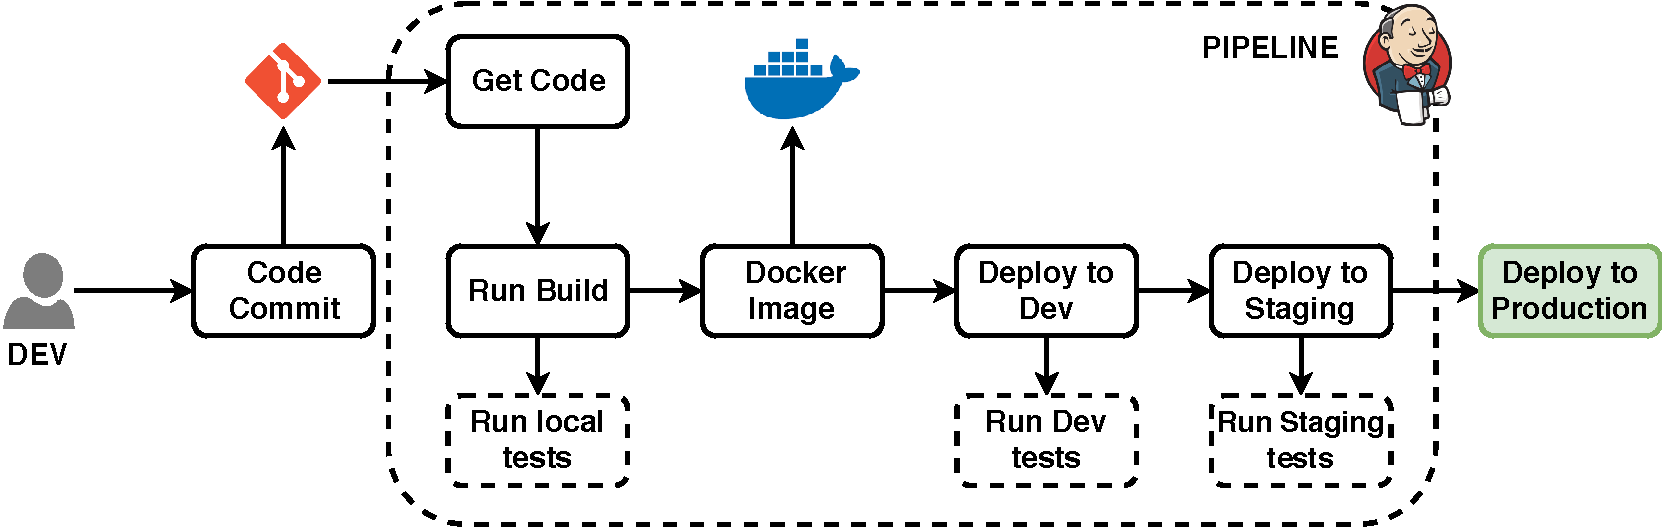
\includegraphics[scale=0.5]{Images/JenkisPipeline.pdf}
	\caption{Example of a Jenkins Pipeline}
	\label{fig:jenkinsPipeline}
\end{figure}

%********************************** %Second Section  **************************************
\section{Process} 

Behavior-Driven Development \cite{BDD} is a set of practices aimed at delivering high quality software while maintaining a stable stream of communication between development team members, stakeholders and users \cite[p.~12]{BDD}. BDD expands on the concept of Test-Driven Development. TDD can be seen as a cycle composed by three phases:

\begin{itemize}
    \item Write a (unsuccessful) test that describes a feature.
    \item Implement the code related to said feature until the test is successful.
    \item Refactor the code.
\end{itemize}

A clear limitation of TDD is the fact that often developers are unsure about the starting point and the scope of the tests they have to write. This phenomenon sometimes leads to test cases being overly specific and strictly bundled to a particular iteration of the code. Simple modifications, like changing test names to complete sentences, allow to maintain a stronger focus of what the software should do (the behavior) rather than the specific method being tested \cite[pg.~14]{BDD}. The point of this approach is to have tests that are more similar to what a specification would look like. Being an highly collaborative procedure (in which information are shared in plain English, or any other language of choice), BDD requires a way to define feature stories and scenarios while still having a sufficient level of automation. A tool commonly used to implement such procedures is Cucumber \cite{Cucumber}. Cucumber is a command-line tool that takes plain language text files (called feature files), analyses them and runs them against the system. These files can be seen as executable specifications that tell the system \textit{what} to do. The features are described by concrete examples that share a common vocabulary understood by all parties. Said files are written using a specific syntax called Gherkin \cite[p.~25]{Cucumber}. Gherkin enables software to derive meaning from plain language files by using a series of specific keywords. A Gherkin file [Algorithm \ref{alg:featureWithScenario}] is organized into:

\begin{enumerate}
  \item \textit{Feature}. To construct some initial documentation regarding the purpose of the document.
  \item \textit{Scenario}. To describe the desired behavior. The feature comes with various concrete examples that describe the reaction of the system in a specific situation. A Scenario is basically a list of steps that have to be executed sequentially. It can either pass or fail and should be able to run on its own without the need of pre-existing data. Scenarios are divided into:
  \begin{itemize}
    \item Context. Defined by the keyword \textit{Given}, it defines the preconditions and prepares the environment.
    \item Event(s). Defined by the keyword \textit{When}, it describes the tested action.
    \item Outcome(s). Defined by the keyword \textit{Then}, it defines the expected outcome.
  \end{itemize}
  
  Each line of the scenario is known as a \textit{step} and can be expanded using the keywords \textit{and} and \textit{but}.
\end{enumerate}

\begin{algorithm}[H]
\SetAlgoLined
\textbf{Feature}: Transfer Order\;
    \hspace{5mm} \textbf{Scenario}: Attempt a transfer without items\;
        \hspace{10mm} \textbf{Given} I have 0 Items in Warehouse\;
        \hspace{10mm} \textbf{When} I create a transfer order\;
        \hspace{10mm} \textbf{Then} an error message is prompted\;
\caption{A Feature with Scenario}
\label{alg:featureWithScenario}
\end{algorithm}


Step definitions are written in Ruby and tell the system \textit{how} to do something. Cucumber scans the feature files looking for patterns previously defined using regular expressions and the \textit{Given} keyword. All the definitions are usually bundled together in a single file.
%********************************** %Third Section  **************************************
\section{Automation}

Continuous Integration \cite{CIBook} is a development practice that revolves around the frequent (daily, o even multiple times per day) merging and integration of code. Said technique is employed to increase the rate of release cycles and to improve quality, reliability and productivity \cite{CIArticle}. The main principle of CI is to keep all the code for a given project in a single shared repository. This is usually achieved using some form of source control tool (like GIT) that the developers can use to access the source code, monitor changes and save modifications. Modern source control systems also allow the use of branches in order to work on various iterations of the product at the same time. Changes to the shared code are handled by an automation server [Figure \ref{fig:CI}] that builds the software when changes are committed by the developers (performing at least a daily or nightly build is usually considered a minimum requirement). An example of such tool is the previously seen Jenkins. Said server can also be used to complete an array of additional tasks (like testing, best practice checking, etc). A CI server is also capable of notifying the developers in case of an unsuccessful build or when problems occurs during the testing stages.

\begin{figure}[ht]
	\centering
	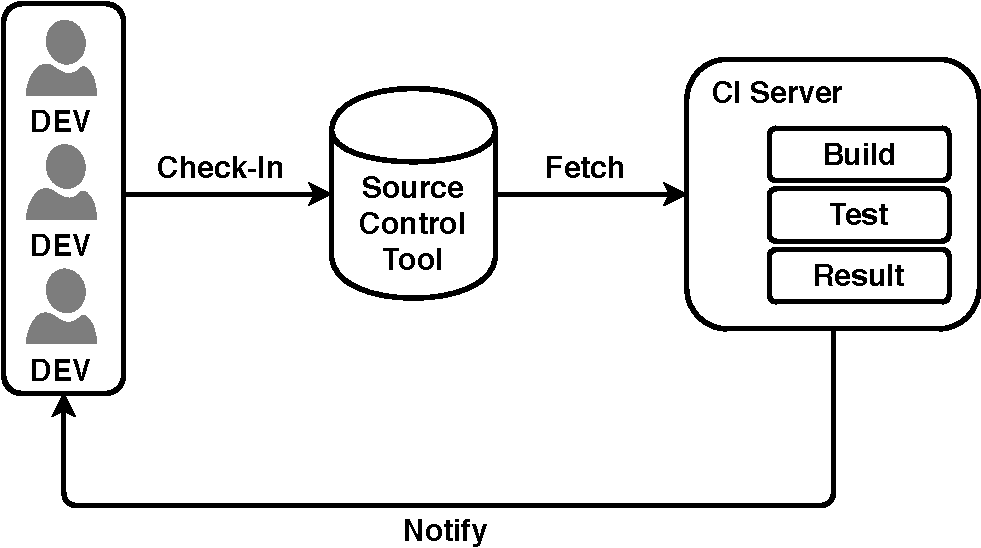
\includegraphics[scale=0.7]{Images/CI.pdf}
	\caption{Continuous Integration}
	\label{fig:CI}
\end{figure}

Although a successful build may already indicate some level of quality in the interested code, additional steps can be taken to further improve code reliability. Despite testing not being necessarily a part of CI, it is usually at least considered within the scope of such techniques. As mentioned before a CI server allows the employment of various testing procedures, including (but not limited to):

\begin{itemize}
    \item Smoke Testing of the core product functionalities.
    \item Unit Testing of individual components (units) like functions, subroutines or methods. 
    \item Integration Testing of multiple software units interacting with each other that are tested to work as group.
    \item Acceptance Testing of the required usage scenarios to the determine to which degree the application meets the specified requirements.
\end{itemize}

The main advantage brought by the employment of CI techniques is naturally the automation of a series of processes that, if executed manually, would introduce the possibility of human error and be very time (and resource) consuming or even impossible to implement effectively. 